\documentclass[10pt,letterpaper]{article}
\usepackage{lmodern}
\usepackage{amssymb,amsmath}
\usepackage{ifxetex,ifluatex}
\usepackage{fixltx2e} % provides \textsubscript
\ifnum 0\ifxetex 1\fi\ifluatex 1\fi=0 % if pdftex
  \usepackage[T1]{fontenc}
  \usepackage[utf8]{inputenc}
\else % if luatex or xelatex
  \ifxetex
    \usepackage{mathspec}
  \else
    \usepackage{fontspec}
  \fi
  \defaultfontfeatures{Ligatures=TeX,Scale=MatchLowercase}
\fi
% use upquote if available, for straight quotes in verbatim environments
\IfFileExists{upquote.sty}{\usepackage{upquote}}{}
% use microtype if available
\IfFileExists{microtype.sty}{%
\usepackage{microtype}
\UseMicrotypeSet[protrusion]{basicmath} % disable protrusion for tt fonts
}{}
\usepackage[margin=0.8in]{geometry}
\usepackage{hyperref}
\hypersetup{unicode=true,
            pdfborder={0 0 0},
            breaklinks=true}
\urlstyle{same}  % don't use monospace font for urls
\usepackage{graphicx,grffile}
\makeatletter
\def\maxwidth{\ifdim\Gin@nat@width>\linewidth\linewidth\else\Gin@nat@width\fi}
\def\maxheight{\ifdim\Gin@nat@height>\textheight\textheight\else\Gin@nat@height\fi}
\makeatother
% Scale images if necessary, so that they will not overflow the page
% margins by default, and it is still possible to overwrite the defaults
% using explicit options in \includegraphics[width, height, ...]{}
\setkeys{Gin}{width=\maxwidth,height=\maxheight,keepaspectratio}
\IfFileExists{parskip.sty}{%
\usepackage{parskip}
}{% else
\setlength{\parindent}{0pt}
\setlength{\parskip}{6pt plus 2pt minus 1pt}
}
\setlength{\emergencystretch}{3em}  % prevent overfull lines
\providecommand{\tightlist}{%
  \setlength{\itemsep}{0pt}\setlength{\parskip}{0pt}}
\setcounter{secnumdepth}{0}
% Redefines (sub)paragraphs to behave more like sections
\ifx\paragraph\undefined\else
\let\oldparagraph\paragraph
\renewcommand{\paragraph}[1]{\oldparagraph{#1}\mbox{}}
\fi
\ifx\subparagraph\undefined\else
\let\oldsubparagraph\subparagraph
\renewcommand{\subparagraph}[1]{\oldsubparagraph{#1}\mbox{}}
\fi

%%% Use protect on footnotes to avoid problems with footnotes in titles
\let\rmarkdownfootnote\footnote%
\def\footnote{\protect\rmarkdownfootnote}

%%% Change title format to be more compact
\usepackage{titling}

% Create subtitle command for use in maketitle
\providecommand{\subtitle}[1]{
  \posttitle{
    \begin{center}\large#1\end{center}
    }
}

\setlength{\droptitle}{-2em}

  \title{}
    \pretitle{\vspace{\droptitle}}
  \posttitle{}
    \author{}
    \preauthor{}\postauthor{}
    \date{}
    \predate{}\postdate{}
  
\usepackage{booktabs}
\usepackage{longtable}
\usepackage{array}
\usepackage{multirow}
\usepackage{wrapfig}
\usepackage{float}
\usepackage{colortbl}
\usepackage{pdflscape}
\usepackage{tabu}
\usepackage{threeparttable}
\usepackage{threeparttablex}
\usepackage[normalem]{ulem}
\usepackage{makecell}
\usepackage{xcolor}
\usepackage{caption, float}

\setlength{\parindent}{15pt}
\setlength{\parskip}{0em}

\begin{document}

\noindent\textbf{Defining constituent order flexibility from a typological perspective: WALS, AUTOTYP, and beyond}

\vspace{1cm}

\noindent How does constituent order vary cross-linguistically, and what drives
this variation? Large-scale typological databases such as WALS (Dryer \&
Haspelmath 2013) and AUTOTYP (Bickel et al. 2017) have focused on
cataloging the dominant constituent orders of the world's languages.
However, languages vary not only in their primary order(s), but also in
the number of additional orders speakers accept and the degree to which
they accept them---their flexibility (Namboodiripad 2017). Here, we
compare the criteria used by each database in determining (non)dominant
constituent order and argue that expanding existing notions of
flexibility can lead to important insights about this variation and its
sources.

Differences in how the databases determine category membership
illustrate the challenges associated with categorical approaches to
constituent order. WALS uses corpus data to determine
\textsc{dominant word order}, which is defined as the order which occurs
at least twice as often as the next most frequent order. If no corpus
exists, a grammar is consulted instead. AUTOTYP, using grammars,
additionally classifies languages as \textsc{rigid}, \textsc{flexible},
or \textsc{free}: rigid languages have exactly one basic order, flexible
languages have a basic order and one or more structurally-conditioned
orders, and free languages have no basic order. There was significant
overlap in the classifications in these databases (N=266; 85\%). Of the
46 non-overlapping languages, 28 (61\%) constituted true disagreements,
8 (17\%) were classified differently from each other due to differing
definitions, and 10 (22\%) were unclear due to the use of different
language varieties.

These differences notwithstanding, the information in such databases can
point us toward potential correlates of flexibility. We aggregated the
constituent order data in WALS and AUTOTYP alongside a set of additional
features we predicted would pattern with flexibility: grammatical
case-marking, argument marking on the verb, the use of head- or
dependent-marking, and the presence of pro-drop. In line with previous
work, we found flexible languages to be somewhat more likely to have
case marking, and rigid languages more likely to lack argument marking
on the verb (Figure \ref{fig:correlates}).

However, manual inspection of AUTOTYP's ``rigid'' category gave us
pause: There is a sense in which many of these languages are not
strictly rigid. For example, Russian is classified as a rigid SVO
language, yet intuitively, it does not pattern with English, another
rigid SVO language; all six orderings of major constituents are
grammatical and attested in Russian (Bailyn 2012), while this is not the
case in English. Likewise, many SOV languages---for example,
Korean---which allow all of the logical constituent orders are
classified as rigid SOV, even though they exhibit considerable
(discourse-mediated) flexibility, as shown in experimental work
(Namboodiripad, Kim, \& Kim 2019).

We conclude with a comparison of three languages classified as SOV
flexible (Avar, Korean, and Malayalam) which nonetheless exhibit subtle
differences in flexibility. We propose that supplementing existing
discrete categories such as ``flexible'' and ``rigid'' with a gradient
notion of flexibility increases descriptive power and, with enough data,
could improve correlational investigations of constituent order
typology.

\hfill Word count: 490

\begin{figure}[b]
\centering

\caption{Correlates of constituent order flexibility}\label{fig:correlates}

\begin{minipage}[c]{0.45\textwidth}

\captionof*{figure}{Argument marking vs. flexibility}\label{fig:flex_marking}

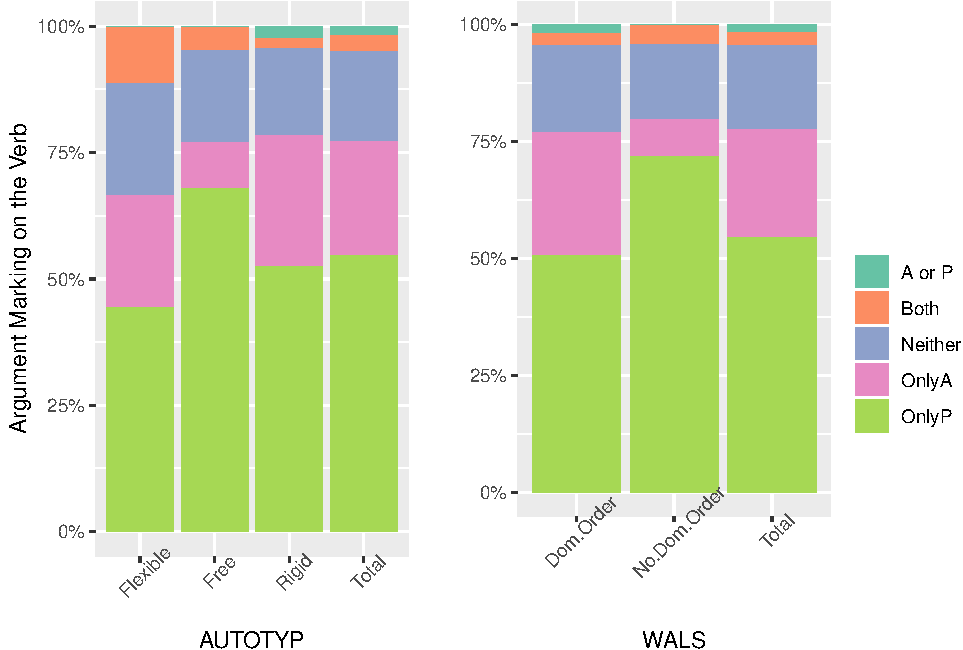
\includegraphics{flexibility_factors_abstract_files/figure-latex/flex_marking-1}

\end{minipage} %
\begin{minipage}[c]{0.45\textwidth}

\captionof*{figure}{Case marking vs. flexibility}\label{fig:flex_case}

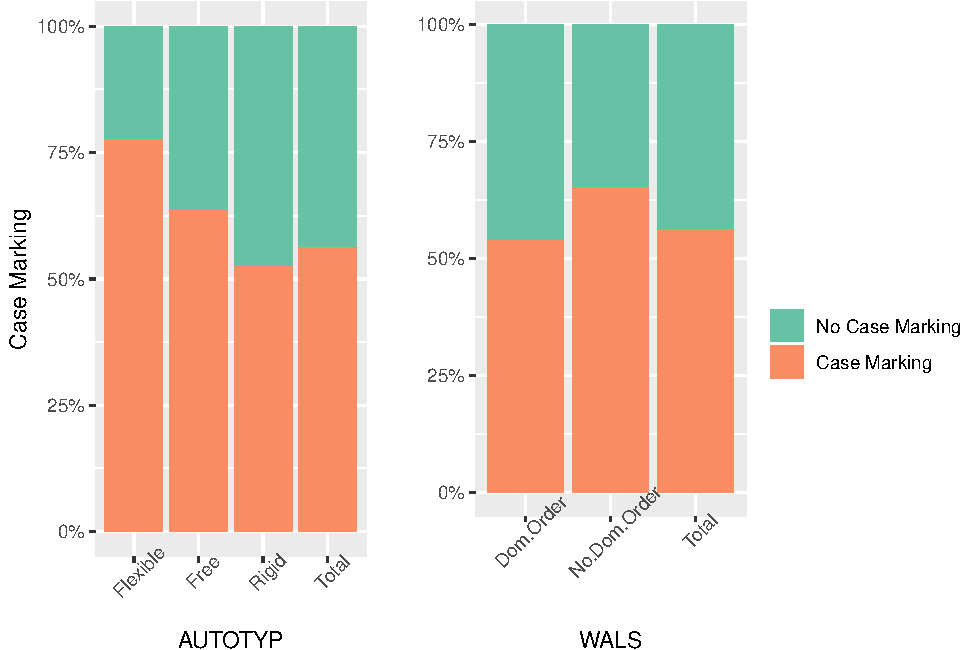
\includegraphics{flexibility_factors_abstract_files/figure-latex/flex_case-1}

\end{minipage}
\end{figure}

\end{document}
